\documentclass[12]{article}
\usepackage{prettyref}
\usepackage[left=2cm,right=2cm,top=2cm,bottom=2cm]{geometry}
\usepackage{graphicx}
\usepackage{bbold}
\usepackage{amsmath, amssymb}
\usepackage{mathtools}
\usepackage{physics}
\usepackage{textcomp}
\usepackage{float}
\usepackage{subcaption}
\usepackage{hyperref}
\hypersetup{
    colorlinks=true,
    linkcolor=blue,
    filecolor=magenta,      
    urlcolor=cyan,
}
\begin{document}
\begin{center}
\begin{Huge}
LANDAU ZENER
\end{Huge}
\end{center}
%\chapter{Landau Zener}\label{ch:LZ}
The Landau-Zener model gives the solution for the dynamics of the magnetization of a 2-level spin system, under the action of slowly reversing external magnetic field at zero temperature [Hans Landau-Zener paper]. Consider, the following single spin- $\frac{1}{2}$ Hamiltonian as an example
\begin{equation}
H_{LZ}(t)=-\Gamma \sigma_x -c t \sigma_z \label{eq:lz1}
\end{equation}
where $\Gamma$ sets the scale of the splitting between the two energy levels, and c is the sweep rate of the applied magnetic field, i.e H(t)=ct. Thus for a field switching its value from $-H_0$ to $H_0$ in time T, $c=\Delta H/T= 2H_0/T$.

Now, for large negative times t, and $\abs{H(t)} \leq \abs{\Gamma}$, $H_{LZ}(t)\approx ct \sigma_z$. Thus, the spin-down state, $\ket{\psi}$ is close to the ground state of the Hamiltonian, as $ct \sigma_z \ket{\downarrow}=-ct \ket{\downarrow}$. As t goes to infinity, $H_{LZ}(t)\approx -ct \sigma_z$, so that the ground state now lies close to the spin up state, as $-ct \sigma_z \ket{\uparrow}=-ct \ket{\uparrow}$. According to quantum adiabatic theorem the state of the system should always lie close to the instantaneous ground state of the Hamiltonian H(t), if the field is changed slowly enough. However, there is a finite probability that the state transits to a higher excited level during the sweep. The probability, p', for this nonadiabatic transition (Landau-Zener tunnelling), as given by the Landau-Zener formula, is
\begin{equation}
p'=exp(\frac{-\pi {\Gamma}^2}{c}) . 
\end{equation}
Therefore, the probability, p, that the state of the system follows instantaneous ground state of the Hamiltonian adiabatically, by changing the magnetization state of the system, in accordance to the reversing field, H(t), is
\begin{equation}
p=1-p'=1-exp(\frac{-\pi {\Gamma}^2}{c}) .   \label{eq:lz2}
\end{equation}

If the energy splitting between the ground state and the first excited state of the Hamiltonian at the anticrossing is denoted by $\Delta E$, then it can be observed that $\Delta E= 2 \Gamma$. Thus, in terms of $\Delta E$, equation(\ref{eq:lz3}) becomes 
\begin{equation}
p=1-exp(\frac{-\pi {\Delta E}^2}{4c}) .   \label{eq:lz3}
\end{equation}

The deviation from the ground state occurs at $H \approx 0$, with a probability p', and is accompanied by a step in the magnetization. This step depends on both the
\begin{figure}[H]
\centering 
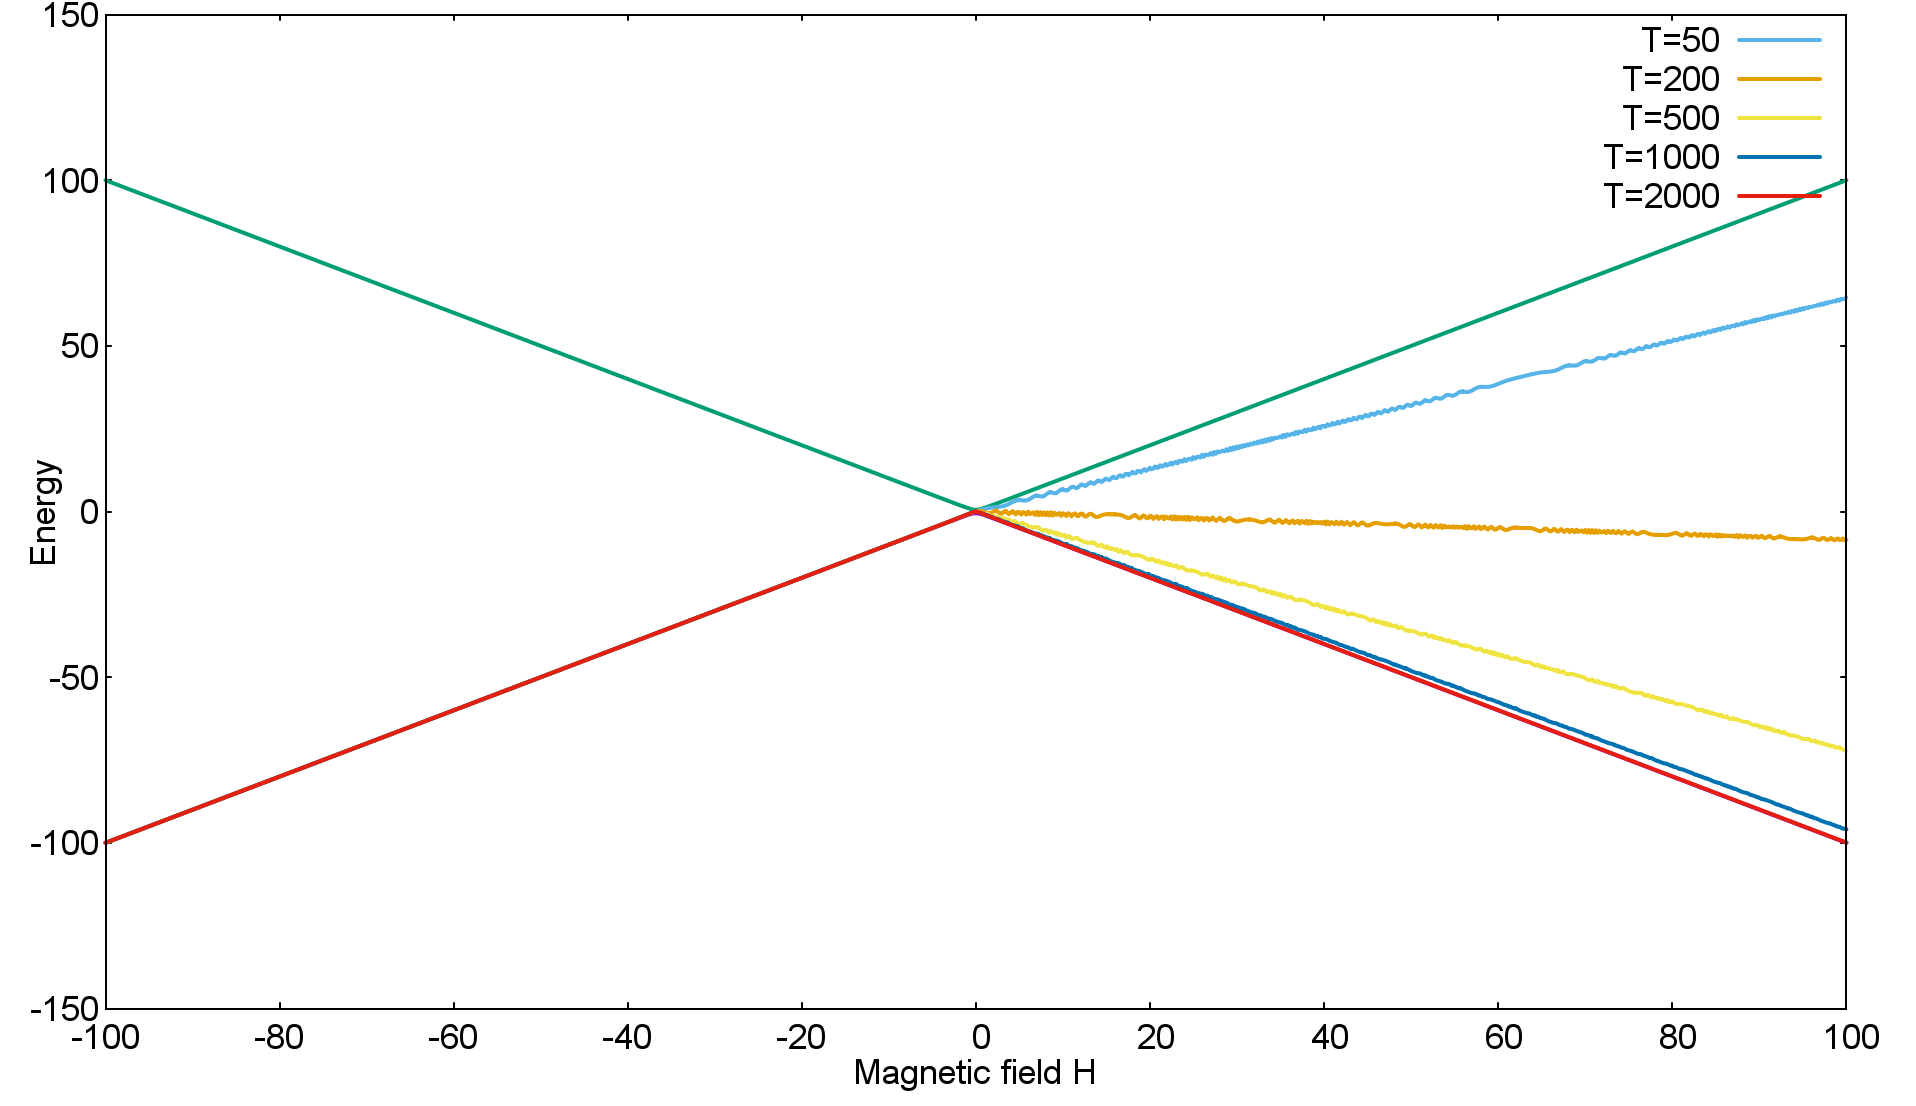
\includegraphics[scale=0.3]{EnergySpec_1spin_H100.png}
\caption{Energy spectrum for single qubit Hamiltonian in equation (\ref{eq:lz1}), with instantaneous energy of the state of the system with different sweeping times. $\Gamma=0.5$, $H_0=100$.}
\label{fig:lz1}
\end{figure}
 energy splitting  $\Gamma$, and the sweep rate c [Hans, On Quantum Simulators and Adiabatic Quantum Algorithms: Sarah Mostame?].\\
For a simple 2-level system where $\Gamma$ is chosen to be 0.5 and the field is swept from a value from -100 to 100, figure (\ref{fig:lz1}) gives the energy spectra for the Hamiltonian in equation (\ref{eq:lz1}).
Figure (\ref{fig:lz1}) also shows the energy evolution of the state of the system corresponding to different times T, chosen for the sweeping the field. As is evident from the figure, the probability of the state of the system staying close to the ground state increases with decreasing speed (increasing T), as expected from (\ref{eq:lz2}). For a sweeping time of T=500, figure (\ref{fig:lz2}) shows the instantaneous magnetization state of the system.
\begin{figure}[H]
\centering 
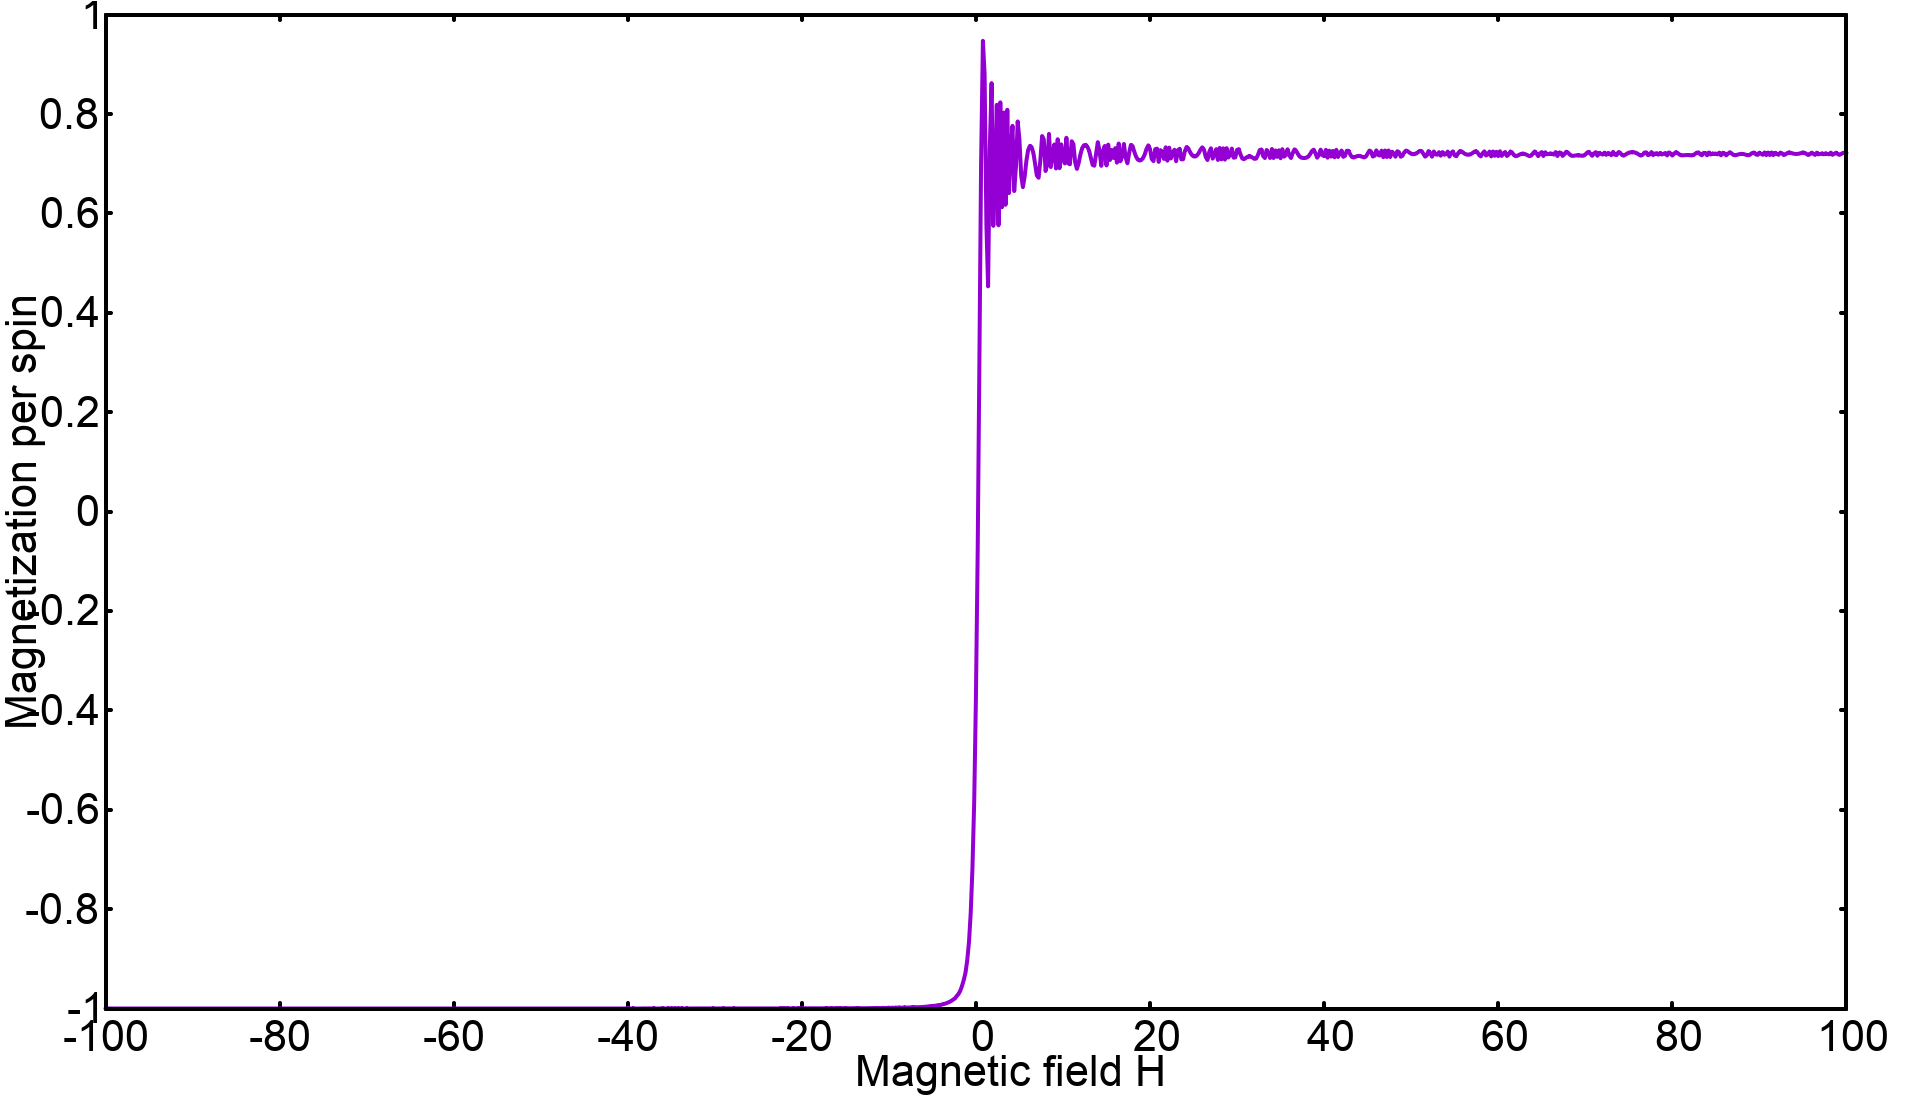
\includegraphics[scale=0.3]{Magnetization_500.png}
\caption{Instantaneous magnetization of the system state for $\Gamma=0.5$, $H_0=100$ and c=0.4.}
\label{fig:lz2}
\end{figure}
Comparing figures (\ref{fig:lz1}) and (\ref{fig:lz2}), it can be observed that the step in the magnetization corresponds to the position of the anticrossing between the ground state and the first excited state in the energy spectrum.\\

For verifying equation (\ref{eq:lz2}), the overlap of the resulting state was computed with the ground state of the Hamiltonian, for different sweeping times. Figure (\ref{fig:lz3}) shows the result obtained.\\

From equation (\ref{eq:lz2}), $p=1-e^{-\frac{\pi \Gamma^2}{2H_0} T}=1-e^{-aT}$, where $a=\frac{\pi \Gamma^2}{2H_0}$. For the chosen parameters, $a$ was calculated to be $3.926 \times 10^{-3}$. This value is found to be in agreement with the value $3.198 \times 10^{-3}$, obtained for the fitting parameter in figure (\ref{fig:lz3}).

\begin{figure}[H]
\centering 
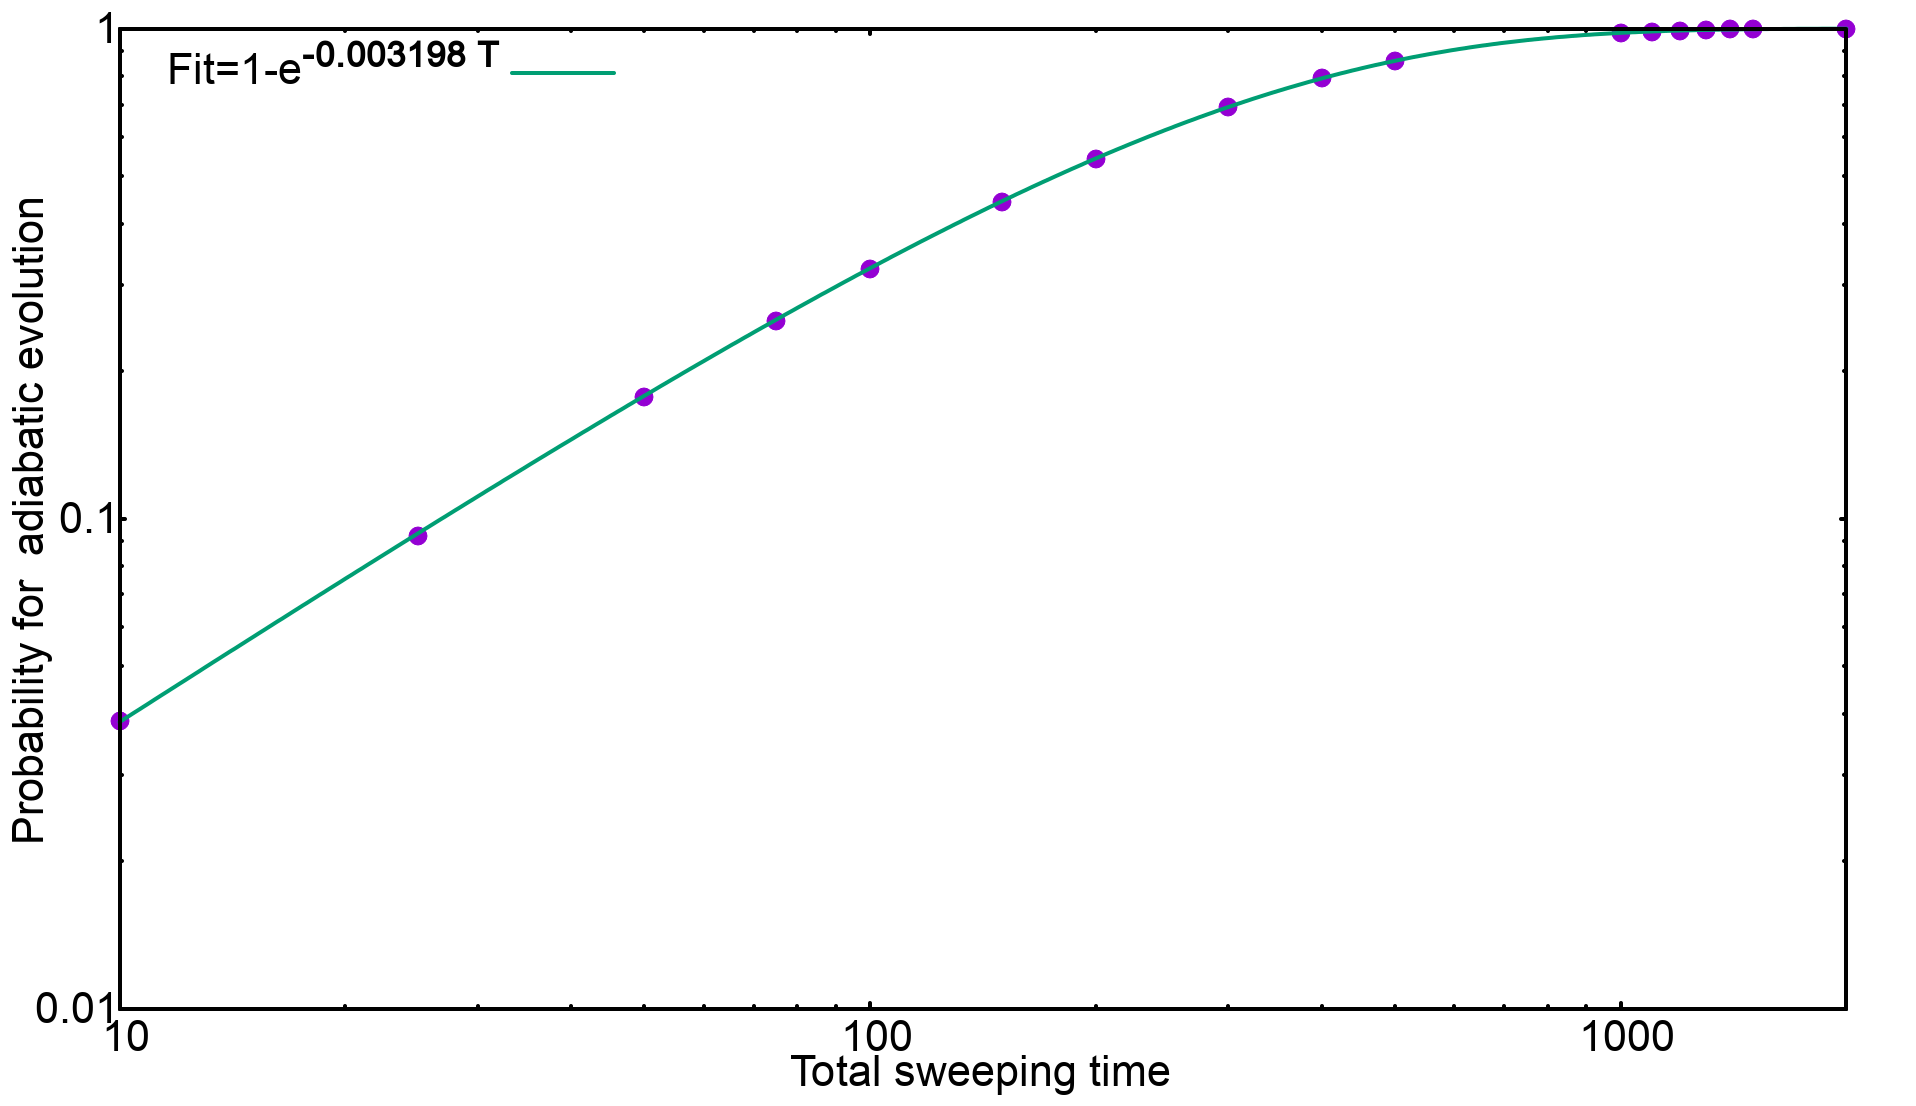
\includegraphics[scale=0.3]{Prob_1spin_H100.png}
\caption{Probability for adiabatic evolution as a function of different sweep times for $\Gamma=0.5$.}
\label{fig:lz3}
\end{figure}



Although both Quantum annealing and Landau-Zener model deal with time dependent Hamiltonians, and the main task consists of studying the evolution of the state of the system under its action, there are two major points of difference. Landau-Zener formula is applicable for 2-level systems, and the process of reversing the magnetic field is ideally carried over an infinite amount of time. On the other hand, quantum annealing problems generally consist of more than two energy levels, and the evolution is carried out for a limited time, i.e. from s=0 to s=1 in terms of the annealing parameter: s.

Despite of these differences, Landau-Zener formula, with minor modifications, can be used as a measure to test if the evolution during the process of quantum annealing is adiabatic. If the dependence of success probability, p, is found to satisfy (\ref{eq:lz3}) the evolution can be regarded as adiabatic.

The Ising model in a transverse field, encoding the optimization problem for quantum annealing involving N variables is one of the simplest microscopic models for uniaxial magnets. Consider, for example, the following Hamiltonian
\begin{equation}
H=-J \sum \limits_{<i,j>} \sigma_i^z \sigma_j^z - \Gamma \sum \limits_i \limits^N \sigma_i^x -H(t) \sum \limits_i \limits^N\sigma_i^z, \label{eq:lz4}
\end{equation} 
where set $<i,j>$ defines the interactions between pairs of spins in the cluster. The modified probability for N spins is then given by [Hans paper, 5-6 reference there]\\
\begin{equation}
p_N=1-p'=1-exp(\frac{-\pi {\Delta E}^2}{4Nc}). \label{eq:lz5}
\end{equation}
Choosing a two spin system, with $\Gamma=0.5$, $J=3$, and $H_0=100$, figure (\ref{fig:lz4}) shows the instantaneous energy spectra as a function of the magnetic field.
\begin{figure}[H]
\centering 
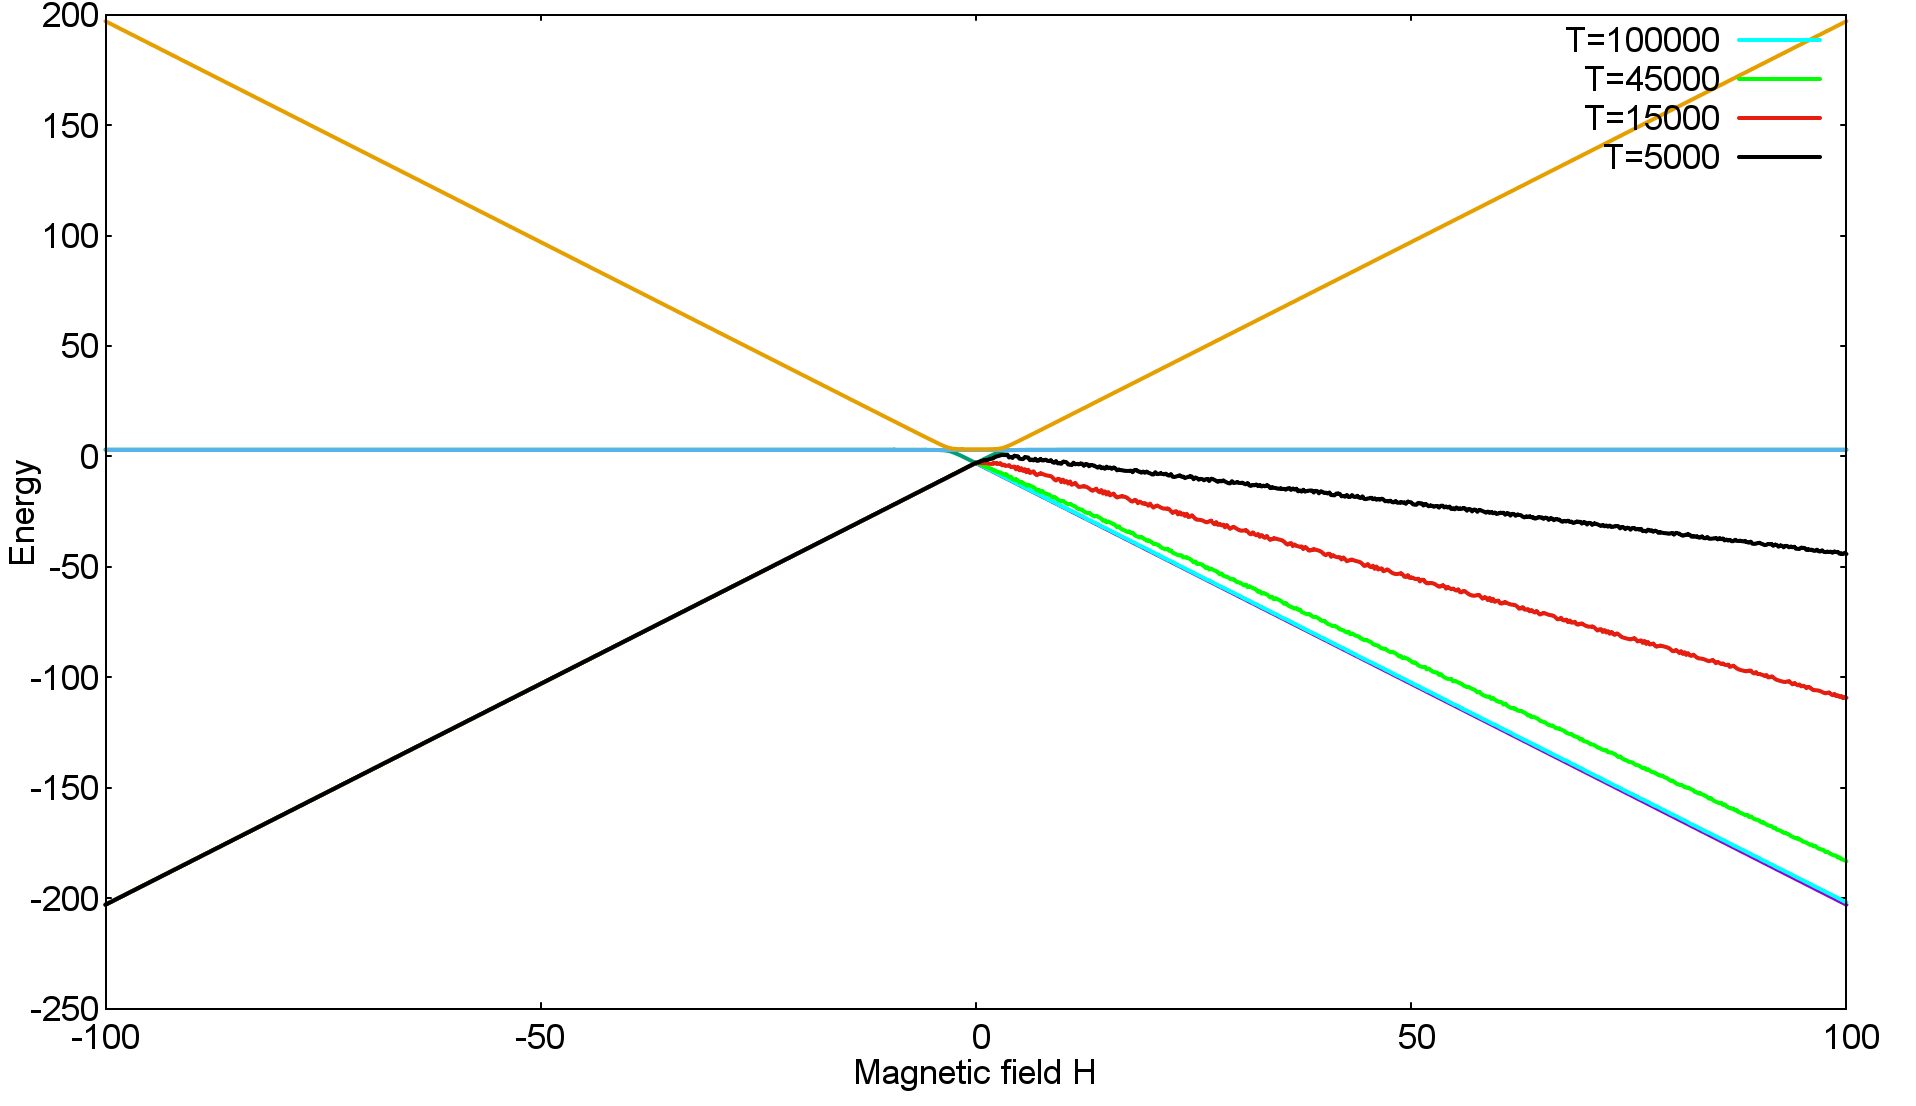
\includegraphics[scale=0.3]{EnergySpectrum_H100.png}
\caption{Energy spectrum for two spin Hamiltonian in equation (\ref{eq:lz4}), with instantaneous energy of the state of the system with different sweeping times. $\Gamma=0.5$, $J=3$, $H_0=100$.}
\label{fig:lz4}
\end{figure}
Figures (\ref{fig:lz5}) and (\ref{fig:lz6}) show the instantaneous magnetization values for two different speeds. Similar to the case of a single spin Hamiltonian, the steps in the magnetization values correspond to the position of anticrossing between the energy levels of the spectrum, in this case as well. Other than the step in the magnetization at $H \approx 0$, in this case, the other step corresponds to the value of H where energy levels become nearly degenerate.

\begin{figure}[H]
  \centering
    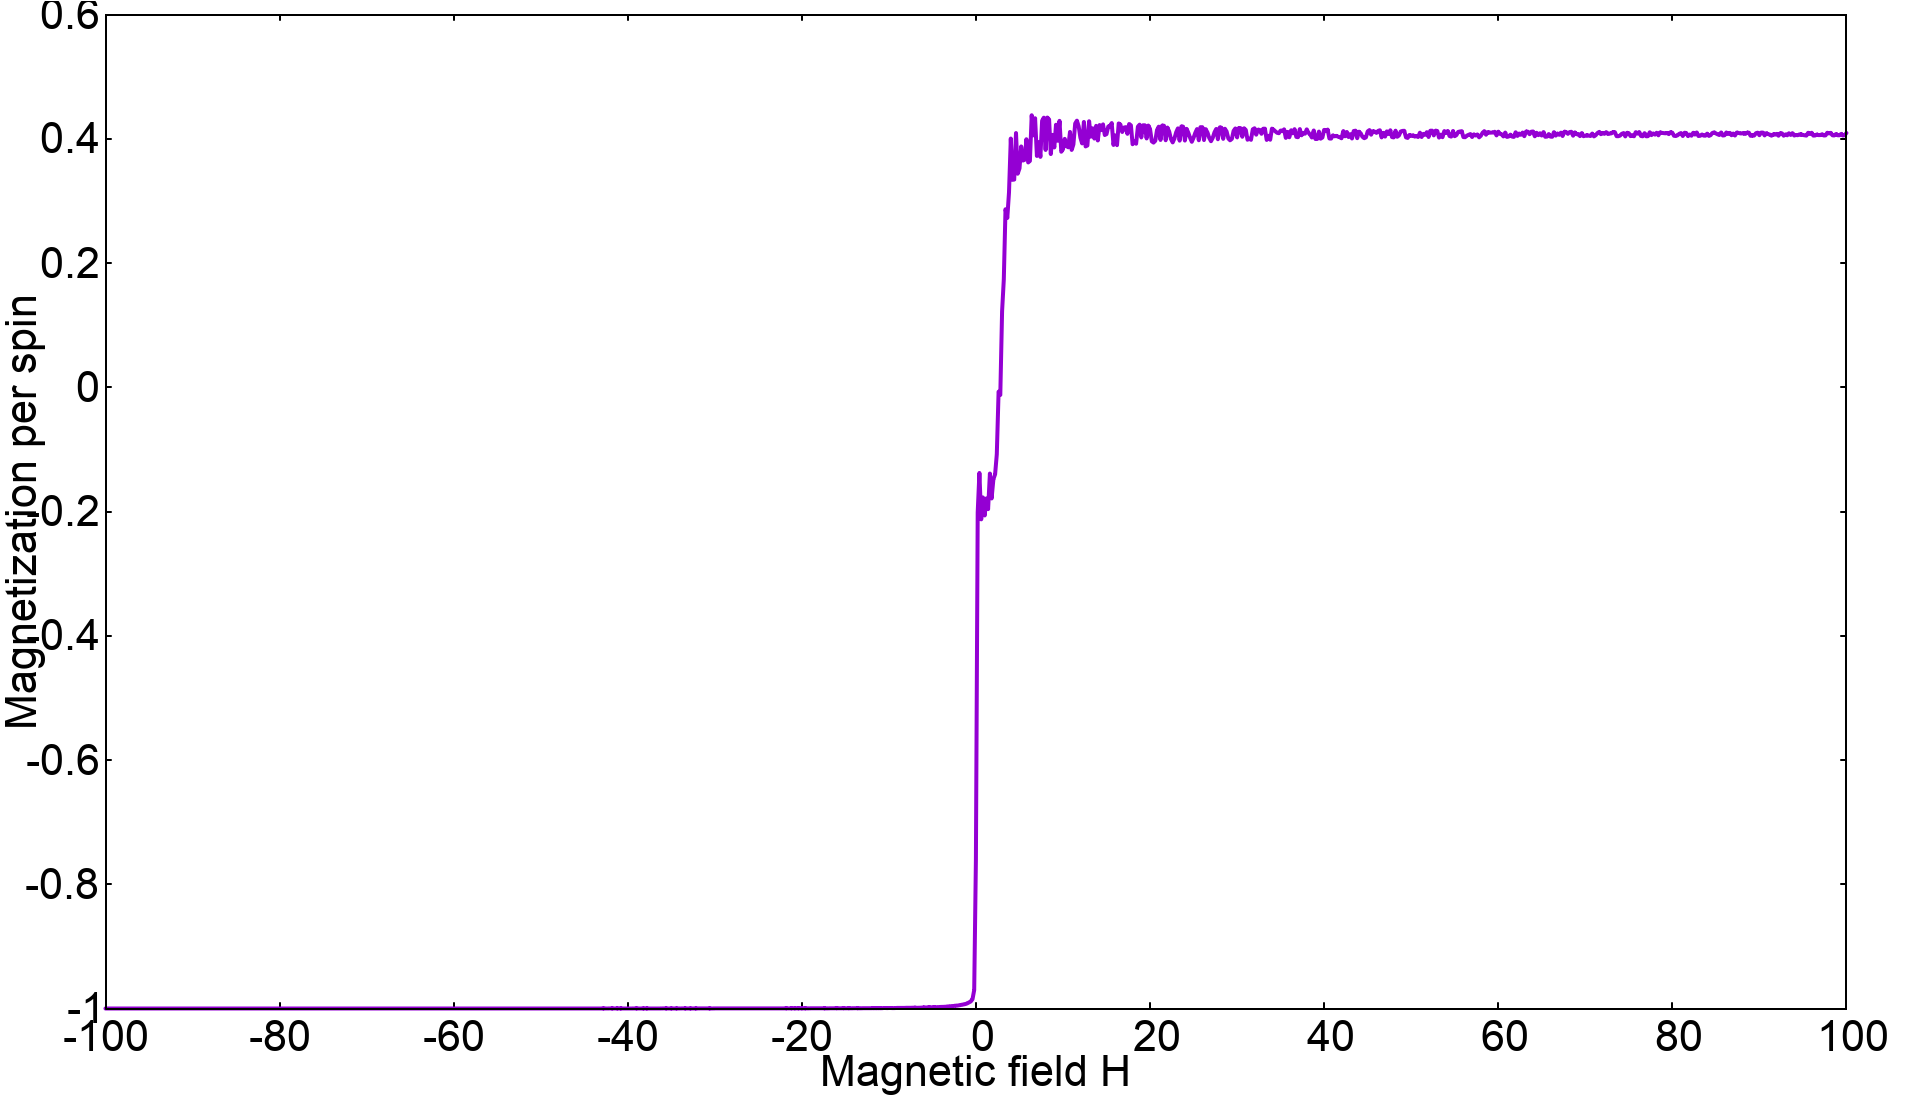
\includegraphics[scale=0.3]{Mag_13_H100.png}
    \caption{Instantaneous magnetization of the system state for $\Gamma=0.5$, $H_0=100$ and c=0.02.}
  \label{fig:lz5}
 \end{figure}
 \begin{figure}[H]
    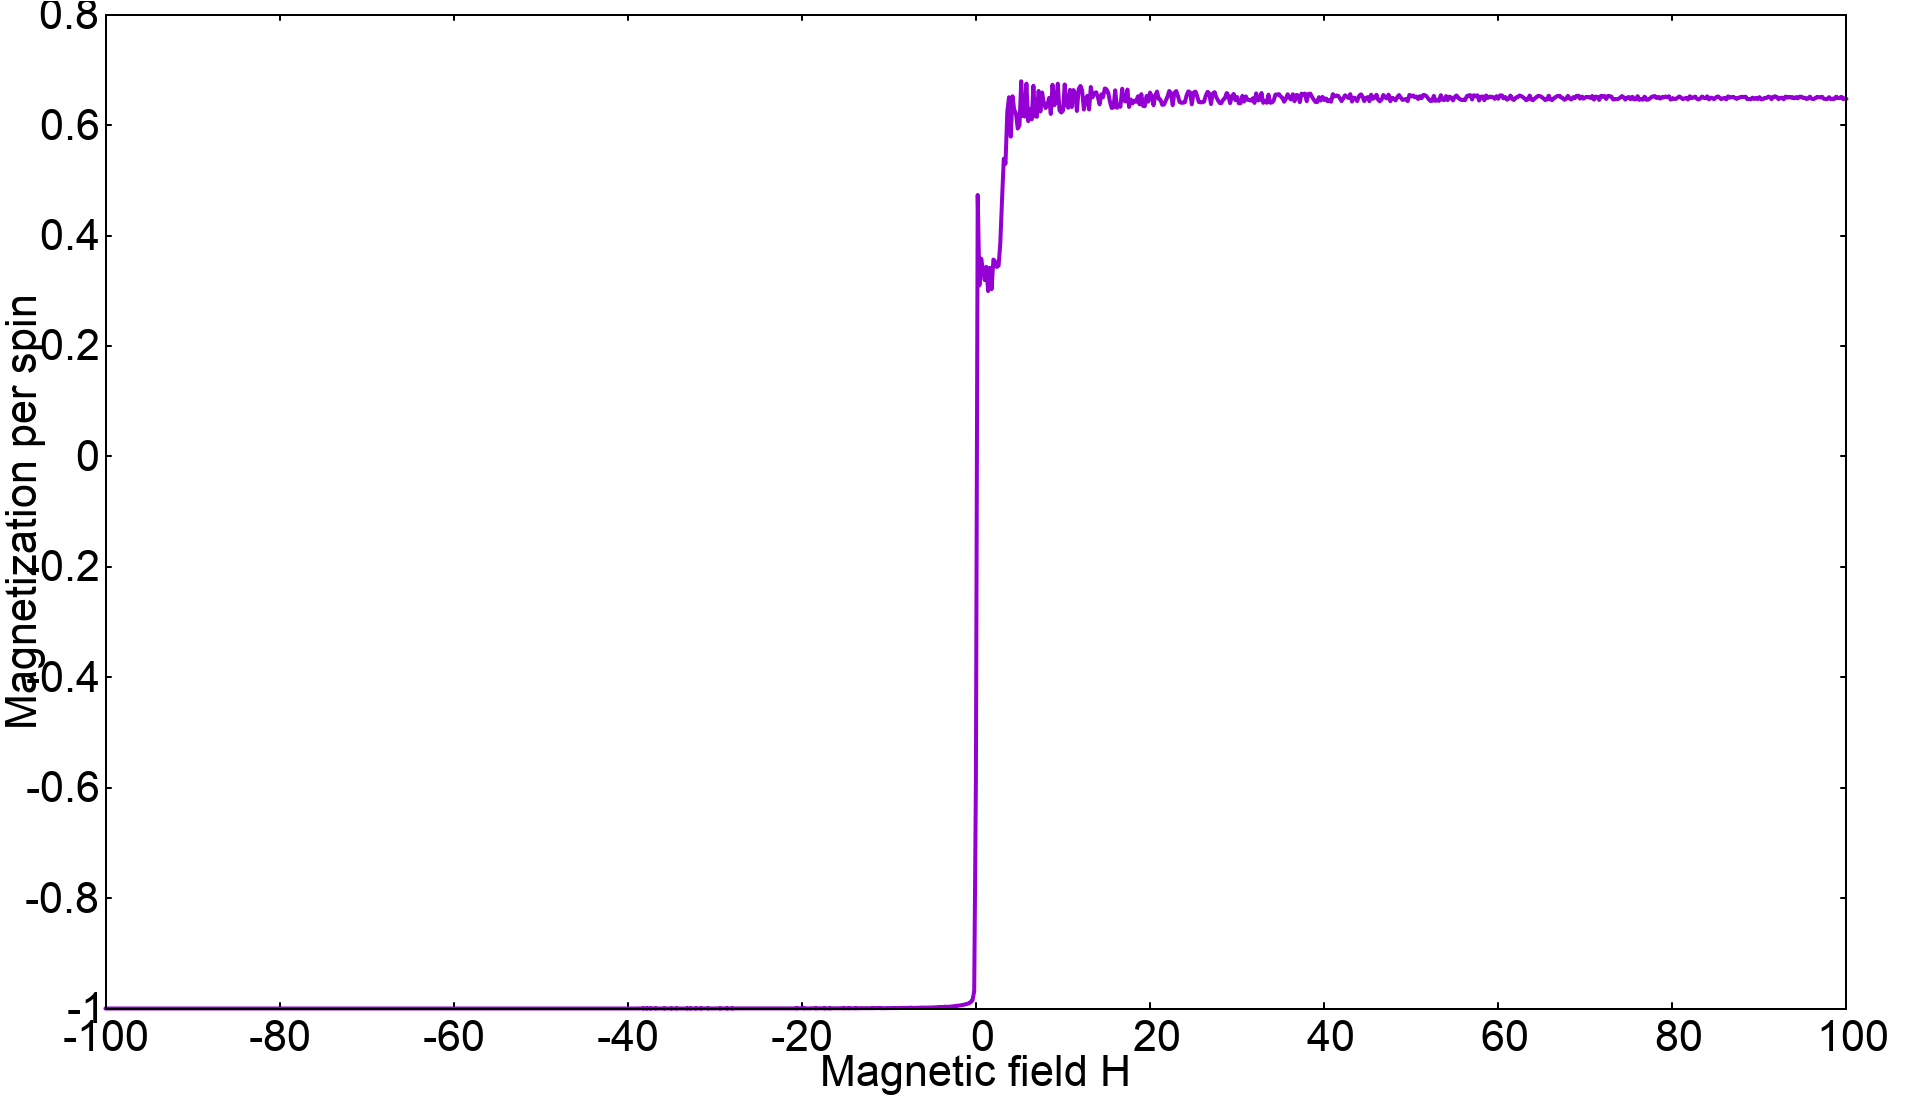
\includegraphics[scale=0.3]{Mag_9_H100.png}
    \caption{Instantaneous magnetization of the system state for $\Gamma=0.5$, $H_0=100$ and c=0.01.}
  \label{fig:lz6}
\end{figure}
On increasing the total time for sweeping the field, i.e. decreasing the sweeping speed, the probability of staying in the ground state, by changing the state of magnetization should increase. This can be confirmed by comparing figures (\ref{fig:lz5}) and (\ref{fig:lz6}).

Finally, for verifying equation ({\ref{eq:lz5}}) the overlap of the resulting state with the ground state is computed for different times. Results obtained are shown in figure (\ref{fig:lz7}). 

The value of minimum gap, $\Delta E$ obtained was 0.162, which results in $a=\frac{\pi \Delta E^2}{8 \Delta H}= 5.182 \times 10^{-5}$. The value of the fitting function obtained in figure (\ref{fig:lz7}) is $5.239 \times 10^{-5}$. Thus, Landau Zener formula is also found to hold for systems having more than two energy levels.
\begin{figure}[H]
\centering 
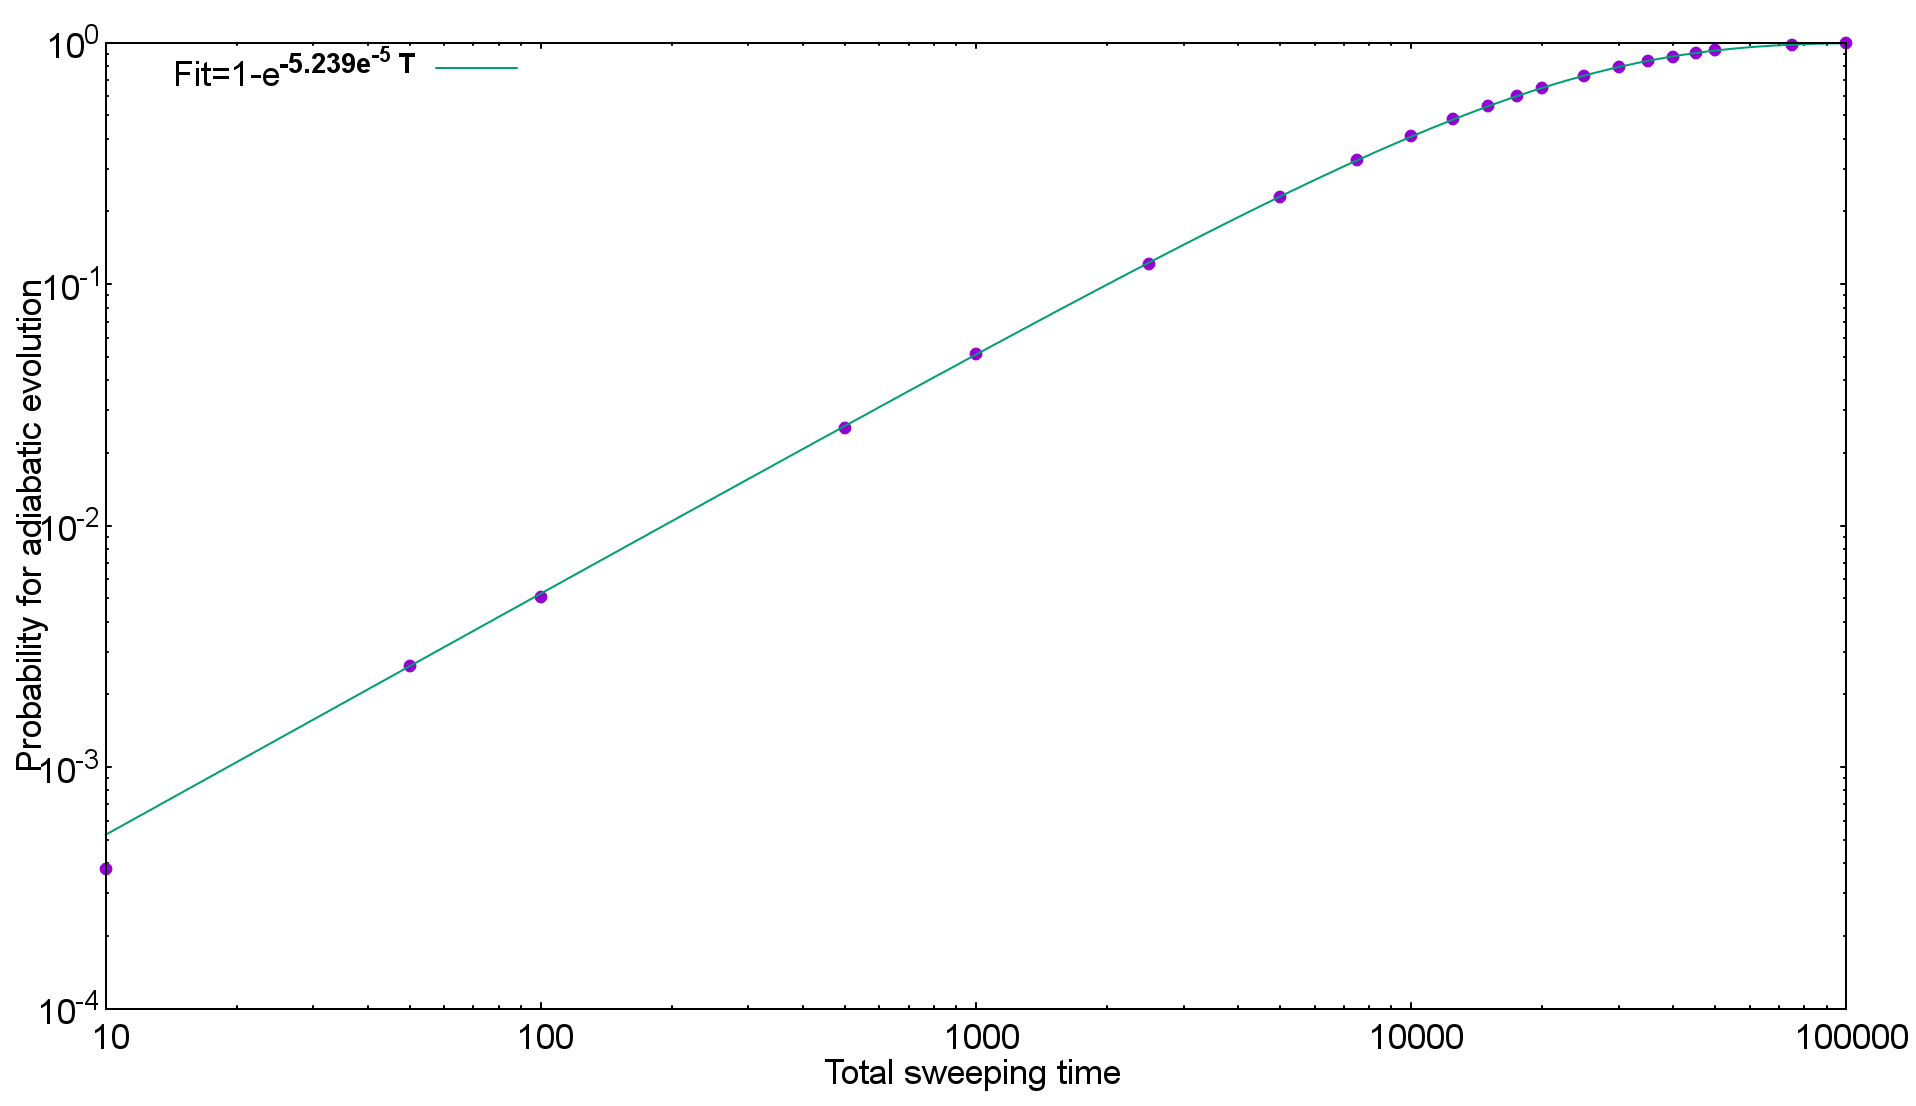
\includegraphics[scale=0.3, width=6.5in]{Probability_H100.png}
\caption{Probability for adiabatic evolution as a function of different sweep times for $\Gamma=0.5$ and $J=3$.}
\label{fig:lz7}
\end{figure}
Equation (\ref{eq:lz5}) will be used again as a check for adiabatic evolution in the subsequent chapters.
\end{document}